\chapter{Preparation of the data}

\textbf{Making the data into frames}

The data acquired from the thermal camera using the Xeneth 2.6 software gives an xvi file as output for each recording. These files was loaded and read into Matlab R2017b as an int16 vector file. Before the frames could be separated from the xvi file, the header in front of the files needed to be excluded. The header contained 307729 data points. With the header removed, the frame separation could be carried out. This was done by first calculating the size of one frame. When knowing that each frame would have the dimensions of 640x480 pixels, the size of one frame would correspond to 307200 data points for each frame. It should be noted that each frame also contained a 16 bit header, so this should be added to the size of each frame. The number of frames was calculated by dividing the length of one frame by the entire length of the data file containing all frames, without the header. By this calculation it was known how many frames the file contained. The data points for each frame was reshaped from a vector into a matrix and verified by showing the images. 
The images contain the pixel intensities of values from -32768 to 32767, which is corespondent to the size of the int16 bit file. 
% or if it is the int16 bit file it's values from 0 to 65535. But the uint16 image looks better and is easier to see, so i think we should use thatone - it won't affect the dataanalysis. 

% Maybe write about temperature convertion

\begin{figure}[H]
	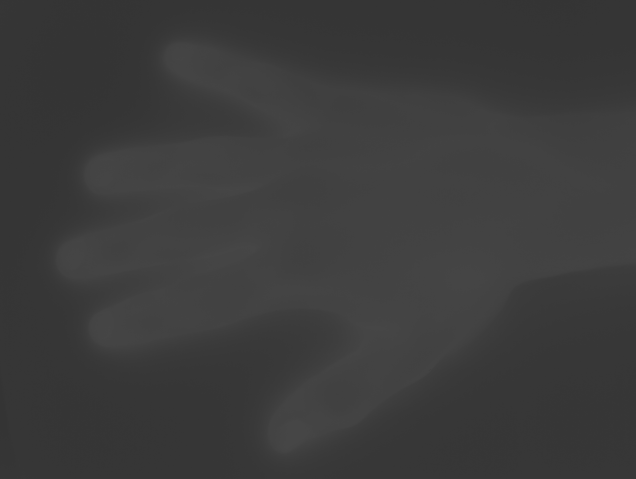
\includegraphics[width=0.6\textwidth]{figures/uint16Hand}  %<--but is not needed.
	\caption{Image of frame one from a subject}
	\label{fig:hand}  %<--give the figure a label, so you can reference!
\end{figure}